\chapter{Blockchain}
Alla base della più moderna forma di commercio, incentrata sulle criptovalute, troviamo una delle forme di commercio più antica mai messa agli atti. Infatti, il viaggio all'interno della Blockchain e le criptovalute ha inizio nel 1400 d.C. in una piccola isola della Micronesia, l'isola di Yap.

\section{La storia della Blockchain}

L'evoluzione della blockchain può essere riassunta nei seguenti passaggi principali mostrati nella tabella temporale \ref{tab:blockchain_evolution}.

Nel 1982, il crittografo David Chaum ha proposto per la prima volta un protocollo simile alla blockchain nella sua tesi del 1982 \textit{"Computer e sistemi creati, mantenuti e resi attendibili da gruppi di individui reciprocamente sospettosi"} \cite{computer_systems_chaum}, da qui in poi li definiamo \textbf{Sistemi di Chaum}. Siamo così difronte alla prima idea di tecnologia blockchain.

\begin{table}[htbp]
  \centering
  \scalebox{1.2}{
    \begin{tabular}{r | @{\foo} l}
      1982 & Sistemi di Chaum \newline \\
      1991 & Timestamp \newline \\
      1992 & Alberi di Merkle \newline \\
      2005 & Bitgold \newline \\
      2008 & Bitcoin \\
    \end{tabular}
  }
  \caption{Evoluzione della Blockchain}
  \label{tab:blockchain_evolution}
\end{table}

\subsection{Introduzione ai Sistemi di Chaum}
Probabilmente, molti degli elementi delle blockchain odierne sono contenuti nel sistema di caveau di David Chaum del 1979, descritto nella sua tesi di laurea del 1982 a Berkeley. Chaum descrive la progettazione di un sistema informatico distribuito che può essere creato, mantenuto e reso attendibile da gruppi di individui reciprocamente sospettosi.

Si tratta di un sistema contenente record in grado di manetere la sicurezza e la privacy dei singoli individui tramite sicurezza fisica. Gli elementi costitutivi di questo sistema includono "caveau" fisici (sicuri), primitive crittografiche (crittografia simmetrica e asimmetrica, funzioni hash crittografiche e firme digitali), e una nuova primitia introdotta da Chaum.

\subsection{Timestamp}
Un ulteriore lavoro su una catena di blocchi protetta da crittografia è stato descritto nel 1991 da Stuart Haber e W. Scott Stornetta \cite{haber1990time}. Essi volevano implementare un sistema in cui i timestamp dei documenti non potessero essere manomessi, oggi considerata la prima applicazione della blockchain.

L'utilizzo del timestamp richiede il superamento di due problematiche:

\begin{itemize}
  \item I dati DEVONO essere contrassegnati con l'ora esatta
  \item Il calendario DEVE essere immutabile
\end{itemize}

I due, idearono una soluzione a queste problematiche, definita "naive", la quale consisteva nell'utilizzo di una \textit{cassetta di sicurezza digitale}. Ogni volta che un cliente ha un documento da marcare temporalmente, lo trasmette a un servizio di marcatura temporale (TSS). Il servizio registra la data e l'ora di ricezione del documento e ne conserva una copia. Se l'integrità del documento del cliente viene messa in discussione, viene confrontata con la copia conservata dal TSS. Se le due copie sono identiche, è la prova che il documento non è stato manomesso dopo la data riportata nei registri del TSS.

Questa procedura soddisfa di fatto il requisito centrale per la marcatura temporale di un documento digitale. Tuttavia, questo approccio solleva diverse preoccupazioni:

\begin{description}
  \item[Privacy] Questo metodo compromette la privacy del documento in due modi: una terza parte potrebbe origliare mentre il documento viene trasmesso e, dopo la trasmissione, il documento è a disposizione del TSS stesso. Il cliente deve quindi preoccuparsi non solo della sicurezza dei documenti che tiene sotto il suo diretto controllo, ma anche della sicurezza dei suoi documenti presso il TSS.
  \item[Larghezza di banda e archiviazione] Sia il tempo necessario per inviare un documento per la marcatura temporale che la quantità di memoria richiesta al TSS dipendono dalla lunghezza del documento da marcare. Pertanto, il tempo e la spesa necessari per la marcatura temporale di un documento di grandi dimensioni potrebbero essere proibitivi. 
  \item[Incompetenza] La copia del documento inviata al TSS potrebbe essere danneggiata durante la trasmissione al TSS, potrebbe essere marcata in modo errato quando arriva al TSS, oppure potrebbe essere danneggiata o persa del tutto in qualsiasi momento mentre è conservata presso il TSS. Ognuno di questi eventi invaliderebbe la richiesta di marcatura temporale del cliente.
  \item[Fiducia] Il problema fondamentale rimane: nulla in questo schema impedisce al TSS di accordarsi con un cliente per affermare di aver apposto la data e l'ora su un documento diverso da quello reale.
\end{description}

Per risolvere queste criticità, Haber e Stornetta, formularono una soluzione: proposero di sottoporre il documento ad un algoritmo di hashing crittografico, ottenendo così un ID univoco ed immutabile del documento.
Semplicemente, anzichè trasmettere al TSS il documento x, viene trasmesso il suo valore \(hash(x) = y\). Per quanto riguarda l'autenticazione, il timestamp di y sarà valido quanto il timestamp di x. Inoltre, questa soluzione riduce drasticamente il problme della larghezza di banda e dell'archiviazione e in più risolve anche il problema della privacy in quanto non viene trasmesso il documento in toto. A seconda degli obiettivi di progettazione, potrebbe essere una singola funzione di hash comune o una per ogni singola utenza.

A ciò si abbinava la firma digitale, utilizzata per identificare in modo univoco il firmatario. Controllando la firma, al client viene garantito che il TSS abbia elaborato la richiesta, che l'hash sia stato ricevuto correttamente e che l'ora inclusa sia corretta. Questo risolve il problema dell'incompetenza da parte del TSS.

Nella figura \ref{fig:blockchain_struttura} è riportata una sequenza d'esempio in cui abbiamo una catena di blocchi connessi da un valore hash.

\begin{figure}[h]
  \centering
  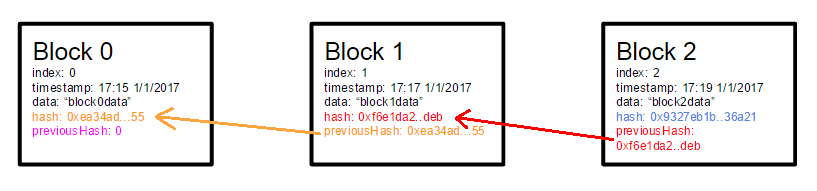
\includegraphics[width=0.8\textwidth]{blockchain_struttura.png}
  \caption{Sequnza di blocchi}
  \label{fig:blockchain_struttura}
\end{figure}

In questa sequenza di blocchi, ogni documento digitale è modificato dai client in diversi istanti di tempo e la catena mantiene un elenco di valori di timestamp relativi agli eventi accaduti sequenzialmente. I valori di timestamp non sono modificabili e in caso di controversie ogni modifica apportata al documento può essere consultata.

\subsection{Alberi di Merkle}
Dave Bayer, contribuì ad integrare la struttura per la marcatura temporale di Haber e Stornetta, con la realizzazione dei Merkle Tree (Alberi di Merkle) \cite{bayer1993improving}, offrendo l'opportunità di raccogliere più documenti in un singolo blocco (Figura \ref{fig:merkle_tree}). Tali alberi ricevono il nome da Ralph Merkle e in essi i nodi foglia sono contrassegnati da un blocco dati, mentre i nodi non-foglia dall'hash crittografico delle etichette dei loro nodi figlio. Detti anche Alberi di hash, mostrano una versione più generica di liste e catene hash e consentono una verifica sicura ed efficace del contenuto di grandi strutture dati.

\begin{figure}[h]
  \centering
  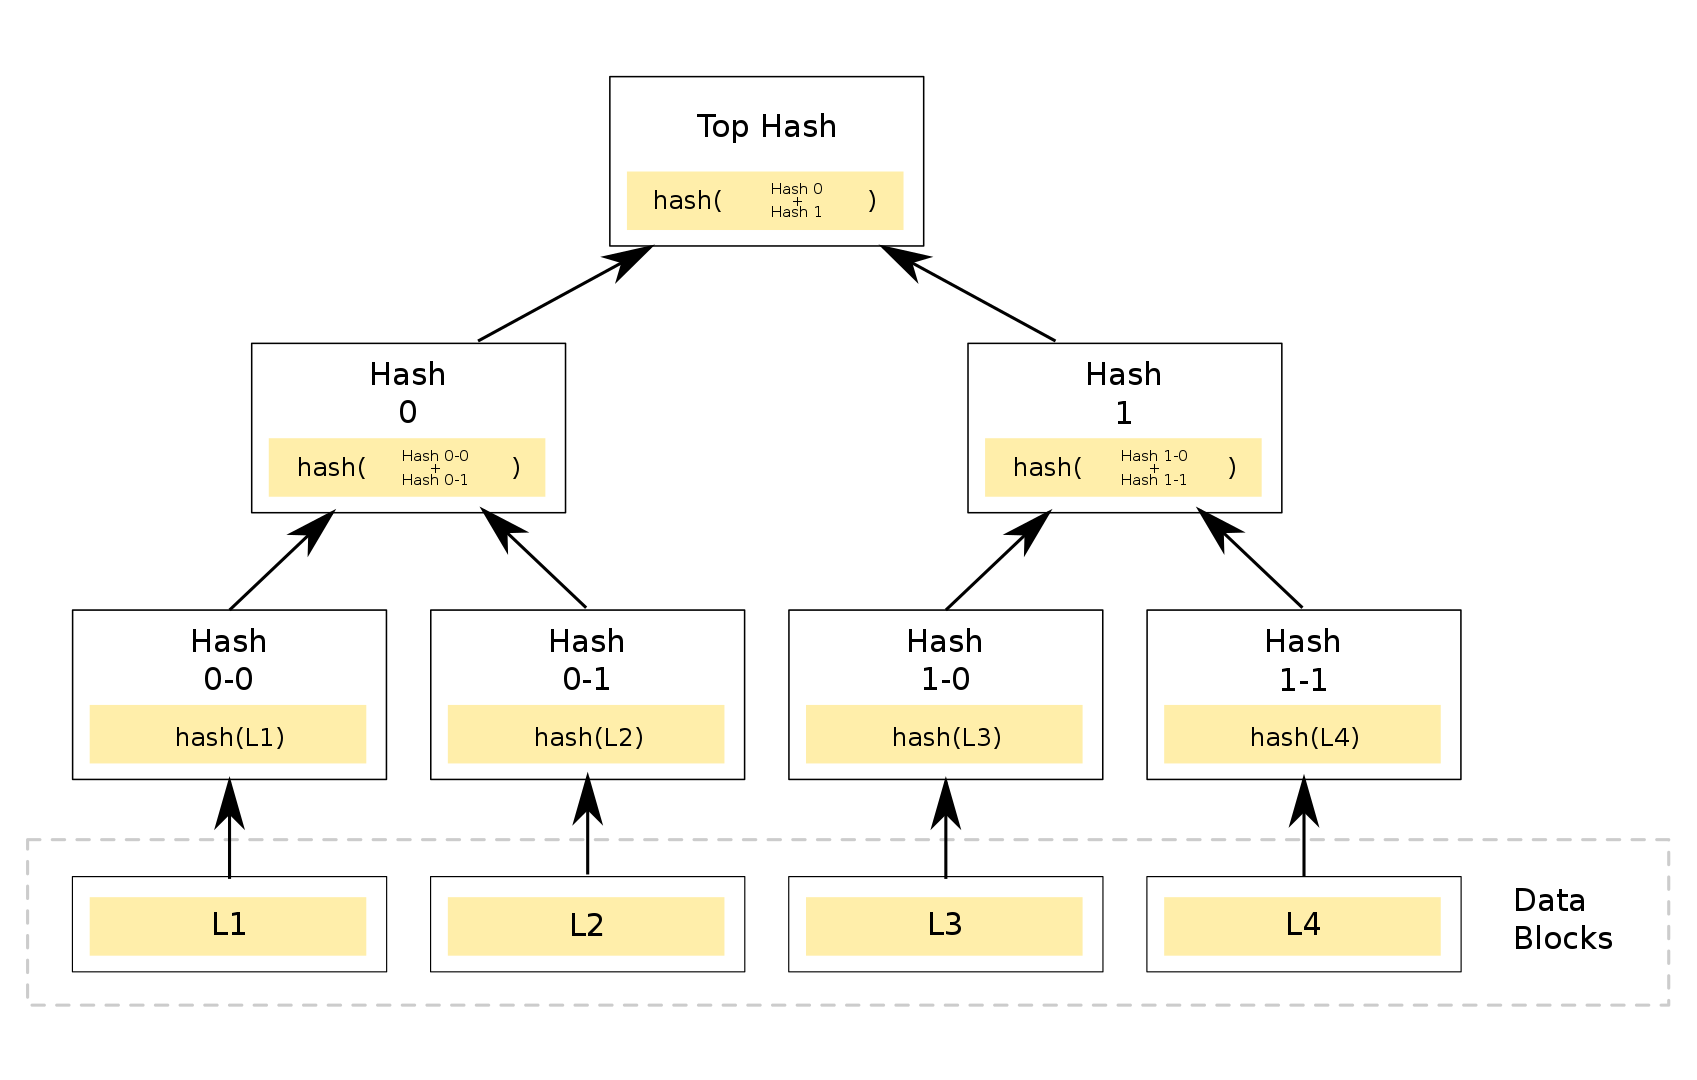
\includegraphics[width=0.9\textwidth]{merkle_tree.png}
  \caption{Esempio di albero di Merkle}
  \label{fig:merkle_tree}
\end{figure}

Nella figura \ref{fig:merkle_tree} possiamo vedere come i valori hash dei blocchi sono definiti "foglie", mentre i valori hash dei loro figli sono detti "nodi". Gli alberi di Merkle vengono utilizzati per rilevare incongruenze tra le repliche e per ridurre al minimo la quantità di dati.

\subsection{Bit gold}
Nel 2005, si ha avuto il primo tentativo di moneta decentralizzata grazie all'informatico Nick Szabo, il quale ha proposto una nuova valuta basata sulla blockchain: \textbf{Bit gold} \cite{szabo_2005}. Moneta che però non ha riscosso molto successo, ma nonostante ciò il 2005 rappresenta un anno cruciale nel contesto blockchain.

La proposta dell'informatico si basa sul calcolo di una stringa di bit a partire da una stringa di bit di sfida, utilizzando funzioni chiamate in vario modo "client puzzle function", "proof of work function" o "secure benchmark function". La stringa di bit risultante è la proof of work.

Ecco le fasi principali del sistema bit gold che Szabo ha definito:

\begin{enumerate}
  \item Viene creata una stringa pubblica di bit, la "stringa di sfida" (vedi passo 5).
  \item Alice sul suo computer genera la stringa di proof of work dai bit di sfida utilizzando una funzione di benchmark.
  \item La proof of work viene registrata in modo sicuro con un timestamp. Questo dovrebbe funzionare in modo distribuito, con diversi servizi di timestamp in modo che non sia necessario affidarsi a un particolare servizio di timestamp.
  \item Alice aggiunge la stringa di sfida e la stringa di proof of work con timestamp a un registro di proprietà distribuito per il bit gold. Anche in questo caso, non si fa affidamento su un singolo server per il corretto funzionamento del registro.
  \item L'ultima stringa creata di bit gold fornisce i bit di sfida per la stringa creata successivamente.
  \item Per verificare che Alice sia la proprietaria di una particolare stringa di bit gold, Bob controlla la catena di titoli non falsificabile nel registro dei titoli di bit gold.
  \item Per verificare il valore di una stringa di bit gold, Bob controlla e verifica i bit di sfida, la stringa di proof of work e il timestamp.
\end{enumerate}

Si noti che il controllo di Alice sul suo bit gold non dipende dal suo solo possesso dei bit, ma piuttosto dalla sua posizione di leader nella catena di titoli non falsificabile (catena di firme digitali) nel registro dei titoli.

Tutto questo può essere automatizzato da un software. I limiti principali alla sicurezza dello schema sono la capacità di distribuire la fiducia nelle fasi (3) e (4) e il problema dell'architettura della macchina, che verrà discusso di seguito.

Hal Finney ha implementato una variante di bit gold chiamata \textbf{RPOW (Reusable Proofs of Work)}. Si basa sulla pubblicazione del codice informatico della "zecca", che viene eseguito su un computer remoto a prova di manomissione. L'acquirente di bit gold può quindi utilizzare l'attestazione remota, che Finney chiama tecnica del server trasparente, per verificare che un determinato numero di cicli sia stato effettivamente eseguito.

Il problema principale di tutti questi schemi è che gli schemi di proof of work dipendono dall'architettura del computer, non solo da una matematica astratta basata su un "ciclo di calcolo" astratto. (Pertanto, potrebbe essere possibile essere un produttore a bassissimo costo (di diversi ordini di grandezza) e inondare il mercato di bit gold. Tuttavia, dal momento che il bit gold è marcato a tempo, il tempo creato e la difficoltà matematica del lavoro possono essere dimostrati automaticamente. Da ciò si può solitamente dedurre il costo di produzione in quel periodo.

A differenza degli atomi d'oro fungibili, ma come nel caso degli oggetti da collezione, una grande disponibilità in un determinato periodo di tempo farà scendere il valore di questi particolari oggetti. Da questo punto di vista, il "bit gold" si comporta più come gli oggetti da collezione che come l'oro. Tuttavia, la corrispondenza tra questo mercato ex post e l'asta che determina il valore iniziale potrebbe creare un profitto molto consistente per il "minatore di bit gold" che inventa e distribuisce un'architettura informatica ottimizzata.

Pertanto, il bit gold non sarà fungibile in base a una semplice funzione, ad esempio, della lunghezza della stringa. Per creare unità fungibili, i commercianti dovranno invece combinare unità di valore diverso.

\subsection{Bitcoin}
Bitcoin nasce ufficialmente agli inizi del 2009 con la creazione del "blocco genesi", ma se ne inizia a parlare nel 2008 a seguito della pubblicazione di un paper scientifico intitolato \textit{"Bitcoin: A Peer-to-Peer Electronic Cash System"} \cite{bitcoin-white-paper}.

\begin{figure}[h]
  \centering
  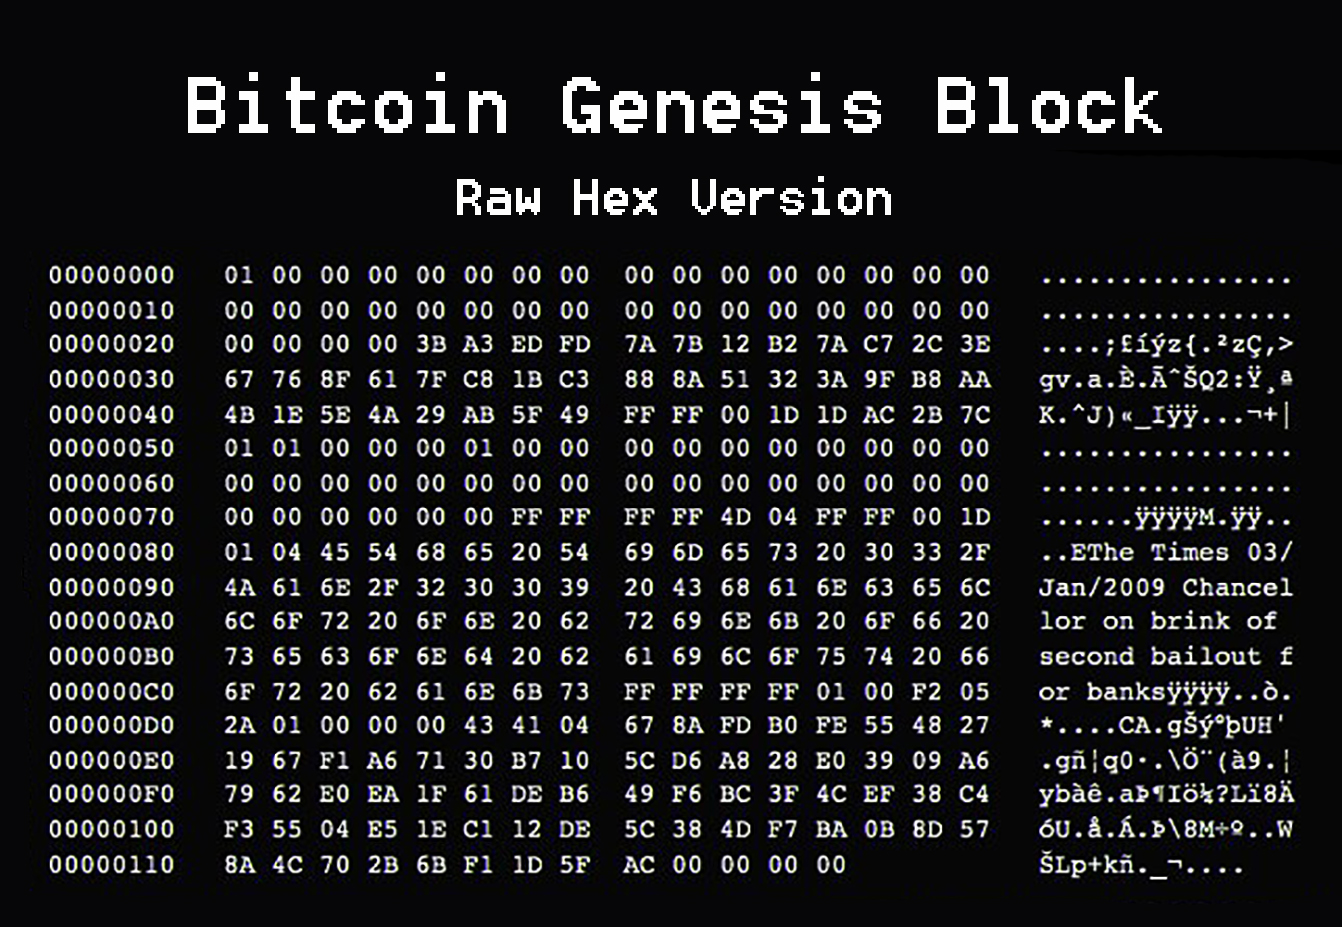
\includegraphics[width=0.9\textwidth]{bitcoin_genesis_block.jpeg}
  \caption{Messaggio di Satoshi Nakamoto incorporato nella coinbase del primo blocco}
  \label{fig:bitcoin_genesis_block}
\end{figure}

Il \textbf{libro bianco o "whitepaper" di Bitcoin} fu pubblicato in un articolo scientifico tramite Cryptography Mailing List nel mese di \textbf{ottobre del 2018}. Essendo pubblicato in modo anonimo sotto lo pseudonimo Satoshi Nakamoto genera ancora più mistero e confusione. Così tanto che ancora oggi si cerca un vero nome dietro quel soprannome.

\textit{Prima di iniziare è bene fare una precisazione: bitcoin con la b minuscola è la moneta digitale, Bitcoin con la b maiuscola è il protocollo che la governa.}

L'obiettivo di Satoshi era quello di creare un sistema di pagamento tramite una versione puramente peer-to-peer di denaro elettronico che permetterebbe di effettuare pagamenti online da un'entità ad un'altra senza passare tramite un'istituzione finanziaria centrale. I nodi peer-to-peer, che costituiscono la rete, non formano gerarchie client-server ma agiscono al contempo sia da client che da server.

Le firme digitali offrono una soluzione parziale al problema, ma i benefici principali sono persi se una terza persona di fiducia è ancora richiesta per prevenire la doppia spesa. Ovvero, quando un utente fa una transazione ci deve essere la garanzia che i soldi appena spesi non possano essere utilizzati una seconda volta per compierne un'altra, problema illustrato in Figura \ref{fig:double_spending}.

La moneta fisica risolve alla radice questo problema non potendo esistere in due luoghi contemporaneamente. In merito ai pagamenti digitali, in un sistema di fiducia centralizzato il problema è gestito da una terza parte che fa controlli su ogni operazione effettuata dagli utenti.

\begin{figure}[htbp]
  \centering
  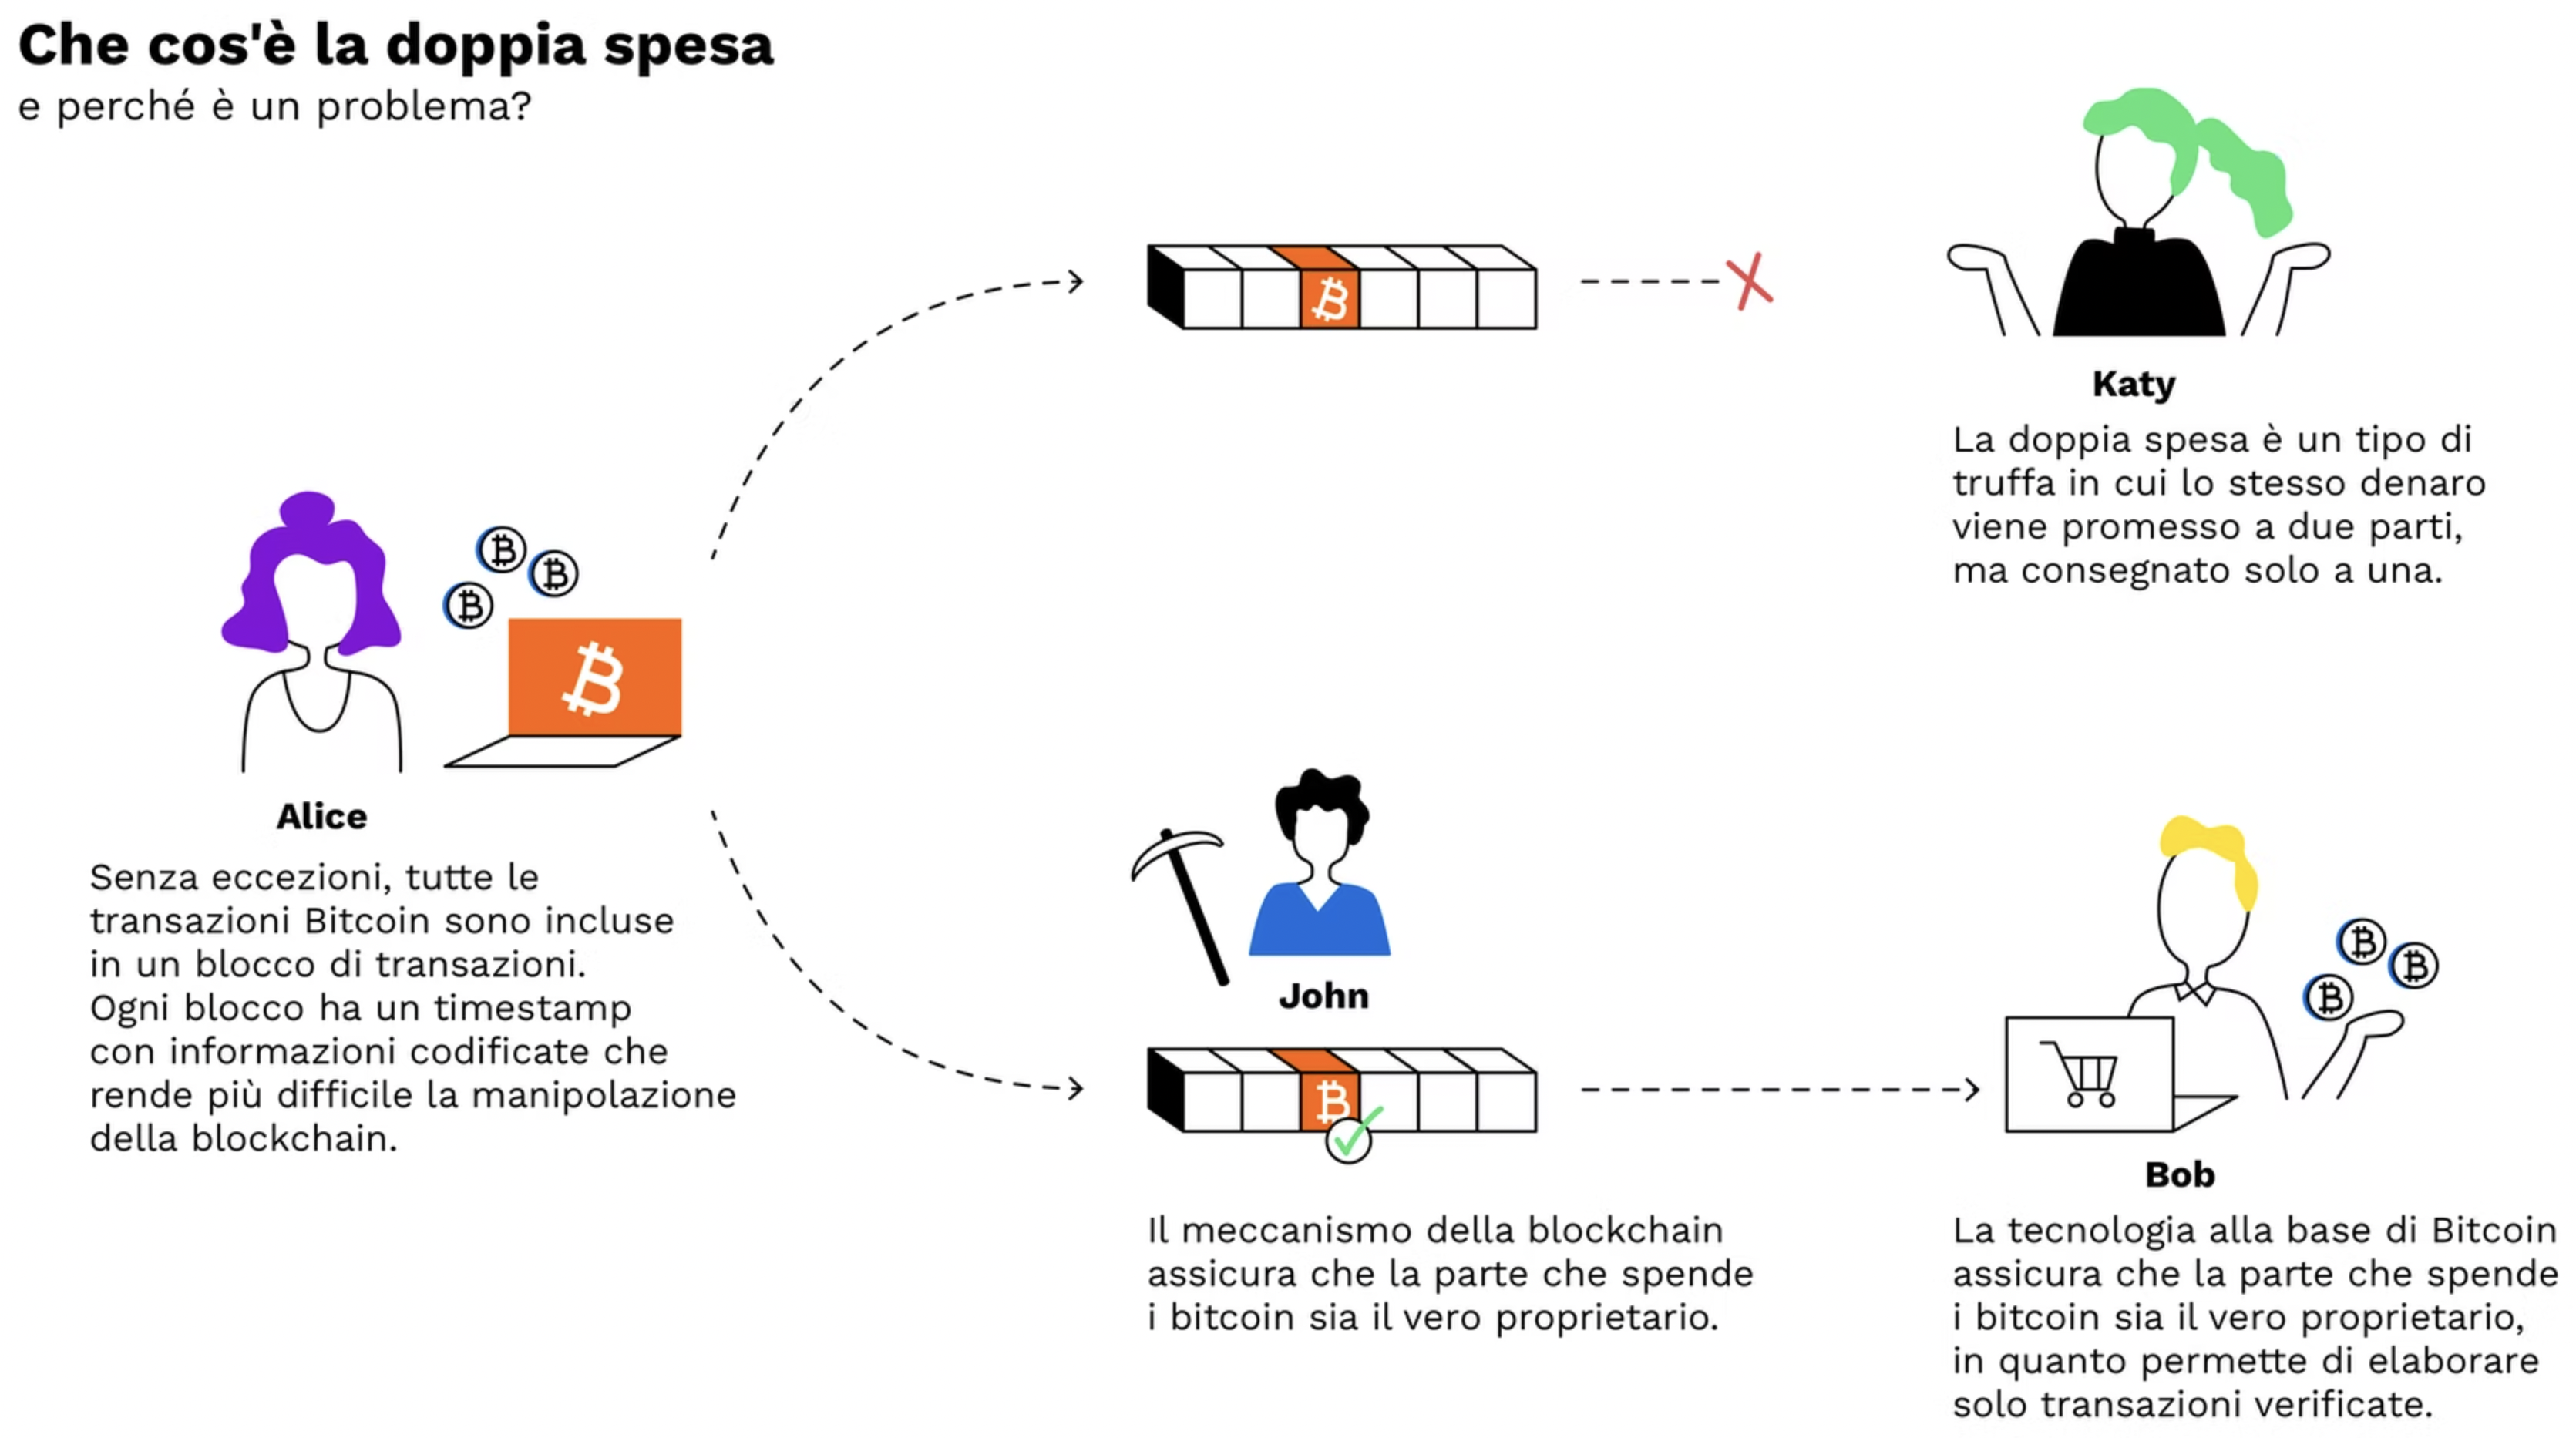
\includegraphics[width=0.9\textwidth]{double_spending.png}
  \caption{Problema del double spending}
  \label{fig:double_spending}
\end{figure}

Satoshi propone una soluzione al problema della doppia spesa mediante l'utilizzo di una rete peer-to-peer, includendo elementi di crittografia.

La legge di mercato della domanda e offerta determinano il valore economico assunto dal bitcoin. Bitcoin è quotato su siti appositi chiamati Exchange. Tali siti permettono di scambiare Bitcoin con Euro, Dollaro Americano o altre monete emesse dai governi, dette anche \textbf{monete fiat}\footnote{Moneta legale (o moneta a corso legale o, ancora, moneta fiduciaria)}. Il primo Exchange è andato online nel marzo del 2010 e quotava bitcoin a soli 0,003\$. Il 22 maggio 2010 vengono acquistate due pizze in Florida per 10.000,00 bitcoin. Meno di un anno dopo la criptomoneta raggiunge il valore di 1,00\$. Nel 2013 la valutazione subisce alti e bassi arrivando a toccare un massimo di 1200,00\$. Con l'apertura di nuovi exchange e grazie alla speculazioni da parte di un numero sempre maggiore di utenti il prezzo sale fino a 10.000,00\$ a novembre 2017. Oggi (fine luglio 2022) ha un valore di 20.893,00\$ circa. L'andamento del bitcoin è illustrato in Figura \ref{fig:bitcoin_quotation}.

\begin{figure}[htbp]
  \centering
  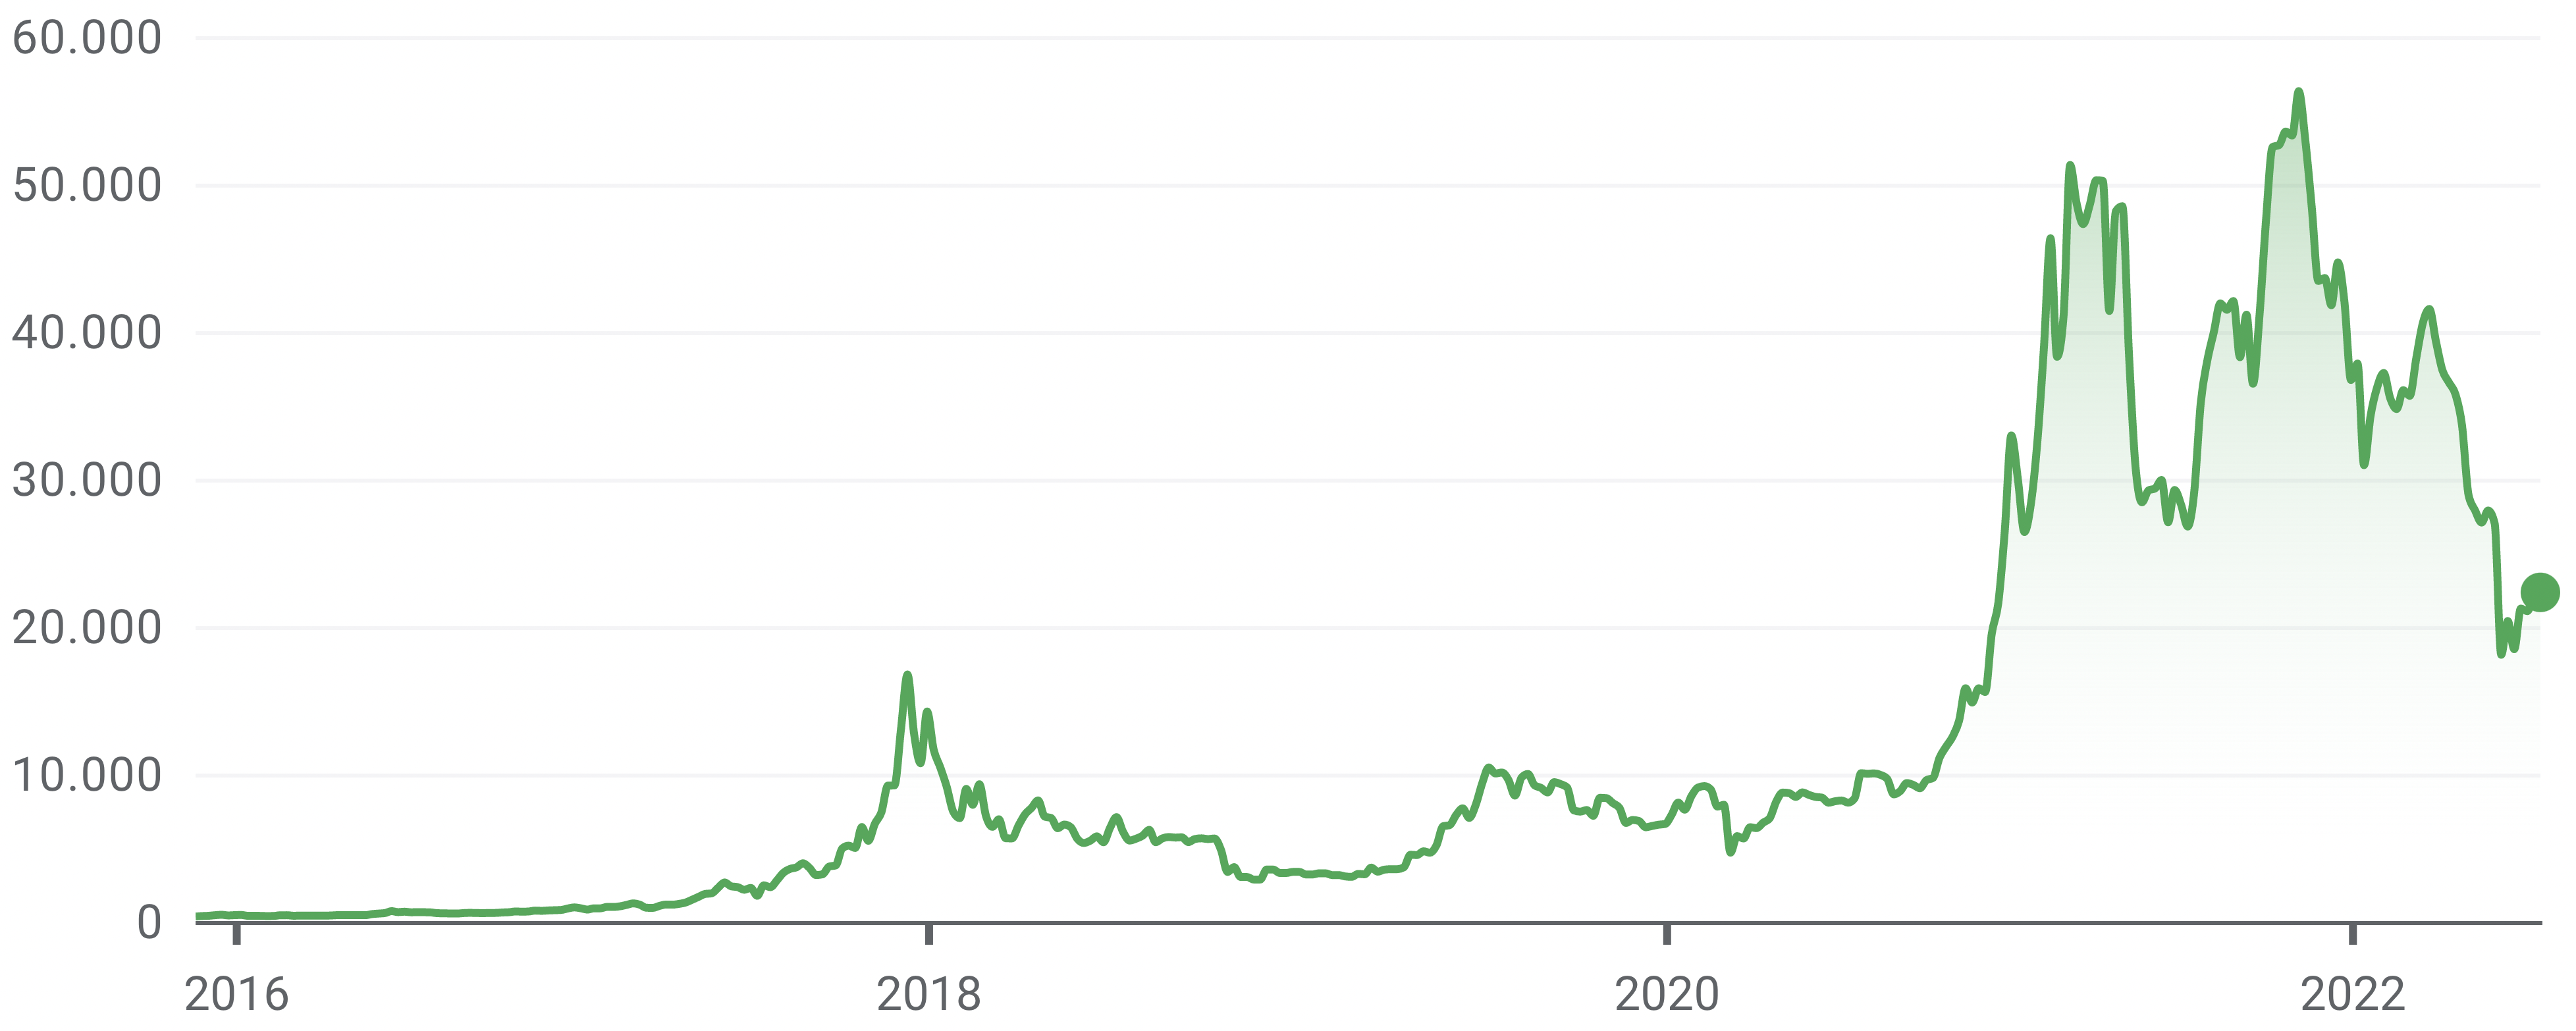
\includegraphics[width=0.9\textwidth]{bitcoin_quotation.png}
  \caption{Andamento del bitcoin}
  \label{fig:bitcoin_quotation}
\end{figure}

\section{Cos'è la blockchain}
La blockchain è una sottofamiglia di tecnologie in cui il registro è strutturato come una catena di blocchi contenenti le transazioni e la cui validazione è affidata a un meccanismo di consenso, distribuito su tutti i nodi della rete nel caso delle \textit{blockchain permissionless o pubbliche} o su tutti i nodi i nodi che sono autorizzati a partecipare al processo di validazione delle transazioni da includere nel registro nel caso delle \textit{blockchain permissioned o private}.

Per alcuni, la blockchain è la nuova generazione di Internet, o meglio ancora è la Nuova Internet. Si ritiene che possa rappresentare una sorta di Internet delle Transazioni arrivndo a creare e rappresentare la Internet del Valore sulla base di sette caratteristiche \cite{bellini_2021}:
\begin{enumerate}
  \item Decentralizzazione
  \item Trasparenza
  \item Sicurezza
  \item Immutabilità
  \item Consenso
  \item Responsabilità
  \item Programmabilità
\end{enumerate}

\subsection{Architettura della blockchain}

\subsection{Come funziona una Blockchain}

\section{Algoritmi di Consenso}

\subsection{Proof of Work}

\subsection{Proof of Stake}

\section{Blockchain pubbliche e private}

\subsection{Blockchain pubbliche}

\subsection{Blockchain private}

\section{Generazioni di Blockchain}

\subsection{Prima generazione: criptovalute}

\subsection{Seconda generazione: digital assets, smart contract e dApp}

\subsection{Terza generazione: scalabilità, interoperabilità e IoT}